\chapter{Implementation}
\label{Implementation}
\textit{This chapter presents the fundamental parts of the implementation process of WebTaint. The chapter starts with a section describing \textit{\nameref{Policies}} enforced by the application. This section is then followed by how \textit{\nameref{souresSS}} was specified and lastly comes the \textit{\nameref{SoftwareArchitecture}} architecture.}



\section{Policies}
\label{Policies}
The development of WebTaint relies on the tasks described in Table \ref{table:taintTracking} in chapter \ref{Background}. These are tainting, detainting, propagating taint, and assertion of non-tainted data. However, to implement the functionality behind the taint tracker needs security policies first be defined. Security policies are principles or actions that the application strives to fulfill \parencite{BayukJenniferL2012Cspg}. The taint tracker developed in this thesis will base on two different aspects. These are \textit{integrity} and \textit{confidentiality}.



\subsection{Integrity}
\label{Integrity}
The integrity policy defines that users may not modify data which they do not have permission to alter. The goal is to ensure prevention of malicious usage of the application where attackers aim to inject malicious executions that can, for example, lead to information disclosure or destruction of application data. To ensure this is the following policy defined:

\hfill
\begin{itemize}
    \item No information or execution of code shall be altered without the users having permission to do so for the given information or execution.
\end{itemize}
\hfill

This entails that no information from sources shall pass through a sink without first being sanitized.



\subsection{Confidentiality}
\label{Confidentiality}
The confidentiality policy defines that data given to the user should only be data that the user have the right to access. The goal is to ensure prevention of malicious usage of applications where attackers aim to steal application data. This gives us the policy:

\hfill
\begin{itemize}
    \item No information shall be released to users without the user having the correct permission for the given information.
\end{itemize}
\hfill

This entails that no information from sources shall pass through a sink unless it has the permission to do so.

\textit{While monitoring confidentiality vulnerabilities are the sources and sinks roles reversed. Meaning that the information to protect is marked as sources and sinks are the systems exit points. The sanitizers are used to specify non-malicious sinks.}



\subsection{Taint Checking}
The integrity policy is enforced by making sure validations, of user input and any data it has come into contact with, are conducted. By enforcing these should preventions of integrity volubilities be reduced severely. The confidentiality policy above is enforced by validating that data from specified sources do not pass through any sink except for those specified as sanitizer as well.

The policies above can be translated into taint policies. These are:

\hfill
\begin{itemize}
    \item Data passing through sources, going into the domain, shall always be marked tainted.
    \item Tainted data is never allowed to pass through sinks.
    \item Predefined sanitizers are the only method calls allowed to detaint data.
\end{itemize}
\hfill



\subsection{Taint Tracking}
Taint checking policies, however, are not the only policies needed to implement WebTaint. WebTaint need policies specifying how the taint tracking should operate. Below are rules defining when taint should propagate:

\hfill
\begin{itemize}
    \item Data resulting in a copy, subset or combination of tainted data shall flag as tainted.
    \item Data disclosing information about tainted data shall flag as tainted.
\end{itemize}
\hfill



\section{Sources, Sinks \& Sanitizers}
\label{souresSS}
Defining the source, sinks, and sanitizers is a large task in itself. There is no official documentation in Java specifying these and depending on the application, framework and library used might this vary a lot.  The sources, sinks and sanitizers used in this thesis is an aggregation from \textcite{sssCodeMaster} and \textcite{sssOWASP}. These web pages present sources, sinks, and sanitizers from their experience with developing web applications. 



\section{WebTaint}
\label{SoftwareArchitecture}
The implementation of WebTaint is divided into three subprojects. These three are Agent, Xboot, and Utils. 

\hfill
\begin{description}
    \item[Agent] Running at runtime and triggers the transformation of sources, sinks, and sanitizers.
    \item[Xboot] Running prior runtime and transforms sources, sinks, sanitizers, String, StringBuilder, and StringBuffer in the base Runtime Environment.
    \item[Utils] Utilities to transform classes into sources, sinks, and sanitizers. 
\end{description}
\hfill

The reasoning behind the division is because of the need of transforming classes both before runtime and during runtime. The Agent is handling the transformation in runtime and Xboot transforms classes on command before runtime. The logic of transforming the classes is, however, the same in both projects and centralized in the Utils project.

Transformation of the String, StringBuilder, and StringBuffer classes, to support tracking of taint, is done in the Xboot project. It is done by iterating through each class and transforming them to: contain a variable to hold the taint flag, and propagate the taint in each method and constructor. The propagation of taint happened when either the taint flag of the class or any of the arguments marked tainted.

The architecture of WebTaint is seen in Figure \ref{fig:WebTaint}. The Java Virtual Machine is un-instrumented and loads WebTaint through the ClassLoader at startup. WebTaint gets access to every class file loaded and instruments the web applications and all needed libraries.

\begin{figure}[H]
    \centering
    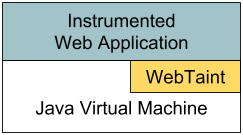
\includegraphics[width=0.4\textwidth]{images/WebTaintArchitecture.png}
    \caption{Architecture of WebTaint}
    \label{fig:WebTaint}
\end{figure}



\subsection{The Utils Project}
The Utils project includes the core logic of marking methods as sources, sinks, and sanitizers. The major part of the implementation is the same for sources, sinks, and sanitizers and the only difference is how they get instrumented if a source, sink or sanitizer is found. The logic behind finding the classes to instrument works by taking all class and matching them with the three criteria below.

\hfill
\begin{itemize}
    \item Is same class as a defined source, sink or sanitizer.
    \item Implements interface of a defined source, sink or sanitizer.
    \item Extends a defined source, sink or sanitizer class (recursive).
\end{itemize}
\hfill

The last item is a recursive call where each extends class is analyzed if it qualifies for any of the three criteria. If a class fulfills, any of the three criteria, are the class instrumented.

The instrumentation of the class works by iterating through each class method and instrumenting them depending on the matching type. Instrumentation of sources will set the return parameter of the method as tainted. Instrumentation of sanitizers works by detainting the return value of the method. For sinks will an assertion call check that none of the method arguments are tainted. If anyone of them is, then a taint exception occurs, and remedial actions conducted. This action should be, depending on options, a logging event, throwing an error or modifying the tainted value into a safe predefined value. During the conducted benchmarking is the option of a predefined value, where the value is an empty string, and logging the event used.



\subsection{Notable Problems}
\label{NotableProblems}
One of the first problems that were introduced during the development of the application was that some classes could not be instrumented during runtime. More precisely, the classes that the Java Virtual Machine relies on can't be instrumented at runtime. However, there is a solution to this. The solution is to pre-instrument the base Java Runtime Environment and create a new instrumented rt.jar file with statically modified versions of the classes. The created jar file loads through the option \textit{Xbootclasspath/p} that appends the classes to the front of the bootstrap classpath. Making the Java Virtual Machine use our modified versions of the base Java Runtime Environment \parencite{xboot} before the original version.

Another problem is that instrumentation of primitives and arrays not possible. It causes a problem since it opens the ability to miss tracking of tainted data if String operations are done with byte- or char arrays. The solution that can solve this is to create shadow as \textcite{BellJ.2014PIdd} did while creating Phosphor \parencite{phosphor}. However, other possible solutions such as creating a centralized memory bank just as \textcite{EnckWilliam2014Taif} did when implementing TaintDroid. They, however, called this shadow memory.

Another problem that emerged was that operations with primitives are direct bytecode translations. Two examples of these are the usage of + (addition) and - (subtraction). Adding operations to these through Javassist's source level API is therefore not possible. To solve this are operations on bytecode level needed. \parencite{Javassist}.